\documentclass[12pt,twoside]{article} 
\usepackage{amsmath, amssymb} 
\usepackage{graphicx}
\usepackage{amsmath} 
\usepackage[active]{srcltx} 
\usepackage{amssymb} 
\usepackage{amscd} 
\usepackage{makeidx} 
\usepackage{amsthm} 
\usepackage{algpseudocode} 
\usepackage{algorithm}
\usepackage[spanish, activeacute]{babel}
\usepackage[utf8]{inputenc}

\renewcommand{\baselinestretch}{1}
\setcounter{page}{1}
\setlength{\textheight}{21.6cm}
\setlength{\textwidth}{14cm}
\setlength{\oddsidemargin}{1cm}
\setlength{\evensidemargin}{1cm}
\pagestyle{myheadings}
\thispagestyle{empty}
\markboth{\small{Pr\'actica 3. Fernando Rivera, Alejandro Contreras}}{\small{.}}

\begin{document}
\centerline{\bf An\'alisis de Algoritmos, Sem: 2020-1, 3CV2, Pr\'actica 3}
\centerline{}
\centerline{04 - 09 -2019}
\begin{center}
\Large{\textsc{Pr\'actica 3: Divide y vencerás}}
\end{center}
\centerline{}
\centerline{\bf {Rivera Paredes Fernando Daniel, Contreras Paredes Alejandro.}}
\centerline{}
\centerline{Escuela Superior de C\'omputo}
\centerline{Instituto Polit\'ecnico Nacional, M\'exico}
\centerline{$ferny036@hotmail.com, acontrerasparedes@hotmail.com$}
\newtheorem{Theorem}{\quad Theorem}[section] \newtheorem{Definition}[Theorem]{\quad Definition} \newtheorem{Corollary}[Theorem]{\quad Corollary} \newtheorem{Lemma}[Theorem]{\quad Lemma} \newtheorem{Example}[Theorem]{\quad Example} \bigskip
\textbf{Resumen:} Análisamos desde otra perspectiva un comportamiento en los algoritmos, sobre dividir un problema general en subproblemas más pequeños, y cómo este tipo
de soluciones ante esa división permite a algoritmos, tanto \textit{Merge}, en su máximo explendor con \textit{Merge Sort}, como uno de los mejores para
ordenamiento.

\centerline{}
{\bf Palabras Clave:} Divide, Vencerás, Logarítmico, Merge, Gráfica
\newpage

\section{Introducción}
Para la siguiente practica se hizo uso del conocimiento obtenido de la recursividad de funciones y la relaci\'on de una con otra se buscara implentar y ver la complejidad 
de los algoritmos merge y merge-sort. como antecedentes tenemos el ´´divide y venceras'' el cual se aplica cuando un problema se resuelve de forma recursiva
de tal manera que el problema principal se descompone en subproblemas del mismo tipo para encontrar un caso base para posteriormente resolverlos y juntarlo para tener soluci\'on del problema orinal


\section{Conceptos B\'asicos} 
\subsection{\textbf{Divide y vencerás}}
\setlength{\parindent}{1.5em}El término Divide y Vencerás en su acepción más amplia es algo más que una técnica de diseño de algoritmos. De hecho, suele ser considerada una filosofía general para resolver problemas y de aquí que su nombre no sólo forme parte del vocabulario informático, sino que también se utiliza en muchos otros ámbitos.
En nuestro contexto, Divide y Vencerás es una técnica de diseño de algoritmos que consiste en resolver un problema a partir de la solución de subproblemas del mismo tipo, pero de menor tamaño. Si los subproblemas son todavía relativamente grandes se aplicará de nuevo esta técnica hasta alcanzar subproblemas lo suficientemente pequeños para ser solucionados directamente. Ello naturalmente sugiere el uso de la recursión en las implementaciones de estos algoritmos.
La resolución de un problema mediante esta técnica consta fundamentalmente de los siguientes pasos:
\begin{enumerate}
  \item En primer lugar ha de plantearse el problema de forma que pueda ser descompuesto en k subproblemas del mismo tipo, pero de menor tamaño. Es decir, si el tamaño de la entrada es n, hemos de conseguir dividir el problema en k subproblemas (donde 1 ≤ k ≤ n), cada uno con una entrada de tamaño nk y donde 0 ≤ nk < n. A esta tarea se le conoce como división.
  \item En segundo lugar han de resolverse independientemente todos los subproblemas, bien directamente si son elementales o bien de forma recursiva. El hecho de que el tamaño de los subproblemas sea estrictamente menor que el tamaño original del problema nos garantiza la convergencia hacia los casos elementales, también denominados casos base.
  \item Por último, combinar las soluciones obtenidas en el paso anterior para construir la solución del problema original.
\end{enumerate}
\centerline{}


\section{Experimentaci\'on y Resultados}
\subsection{\textbf{Planteamiento de los distintos problemas}}
Para el desarrollo de la práctica planteamos dar solución a un problema de ordenamiento con el algoritmo de \textit{Merge Sort}; sin embargo, para implementarlo, es necesario
desarrollar el algoritmo de \textit{Merge}, lo que se pretende demostrar es:
$Merge \in \Theta (n)$ y $Merge Sort \in \Theta (n \log (n))$
\centerline{}
\subsection{\textbf{Soluci\'on al primer problema}}

Para el desarrollo del algoritmo de \textit{Merge} se propuso el \textbf{Algoritmo 1}

\begin{algorithm}
  \caption{Merge}\label{euclid}
  \begin{algorithmic}[1]
  \Function{Merge}{$A[0, ..., n-1], p, q, r$}
      \State $n\gets q - p + 1$ \Comment $O(1)$
      \State $m\gets r - q$ \Comment $O(1)$
      \State $I[n]$ \Comment $O(1)$
      \State $D[n]$ \Comment $O(1)$
      \State $i\gets j \gets 0$ \Comment $O(1)$
      
      \For{$i=0 $ \textbf{to} $i \leq n - 1$} \Comment $O(n)$
        \State $I[i]\gets A[p+i]$ \Comment $O(1)$
      \EndFor

      \For{$j=0 $ \textbf{to} $j \leq m - 1$} \Comment $O(n)$
        \State $D[j]\gets A[q+j+1]$ \Comment $O(1)$
      \EndFor

      \State $i\gets j \gets 0$ \Comment $O(1)$

      \For{$k=p $ \textbf{to} $k \leq r$} \Comment $O(n)$
        \If{$i\leq n-1 \land j\leq m-1$} \Comment $O(1)$
          \If{$I[i]\leq D[j]$} \Comment $O(1)$
            \State $A[k] \gets I[i]$ \Comment $O(1)$
          \Else \Comment $O(1)$
            \State $A[k] \gets D[j]$ \Comment $O(1)$
          \EndIf \Comment $O(1)$
          \State $k++$ \Comment $O(1)$
        \Else  \Comment $O(1)$
          \If{$i\geq n$} \Comment $O(1)$
            \While{$j\leq D.length$} \Comment $O(1)$
              \State $A[k] \gets D[j]$ \Comment $O(1)$
              \State $k++$ \Comment $O(1)$
              \State $j++$ \Comment $O(1)$
            \EndWhile
            \Else
              \While{$i\leq I.length$} \Comment $O(1)$
                \State $A[k] \gets I[i]$ \Comment $O(1)$
                \State $k++$ \Comment $O(1)$
                \State $i++$ \Comment $O(1)$
              \EndWhile
          \EndIf
        \EndIf
      \EndFor

      \State \textbf{return} $A$
  \EndFunction
  \end{algorithmic}
\end{algorithm}

Donde podemos ver distintas sentencias \textit{for}, la cuales se encuentran independientes una respecto a la otra, por tanto, de 
manera simplificada podremos llegar a una forma de ecuación tal que:

\centerline{$T(n) = 5*O(1)+O(n)+O(n)+O(n)[18*O(1)]$}
\centerline{}
\centerline{donde: $O(g(n))_{1} + O(g(n))_{2}+\cdots+O(g(n))_n = O(g(n))$}
\centerline{}
\centerline{$\Rightarrow T(n) = O(1) + O(n)+ O(n)[O(1)]$}
\centerline{}
\centerline{donde: $O(f(n)) * O(g(n))= O(f(n)*g(n))$}
\centerline{}
\centerline{$\Rightarrow T(n) = O(1) + O(n)$}
\centerline{}
\centerline{donde: $O(f(n)) + O(g(n)) = O(h(n))$}
\centerline{y $h(n)$ es la funci\'on con mayor jeraqu\'ia respecto a $g(n)$ y $f(n)$}
\centerline{}
\centerline{$\therefore T(n) \in O(n)$}

\begin{figure}
  \centering
    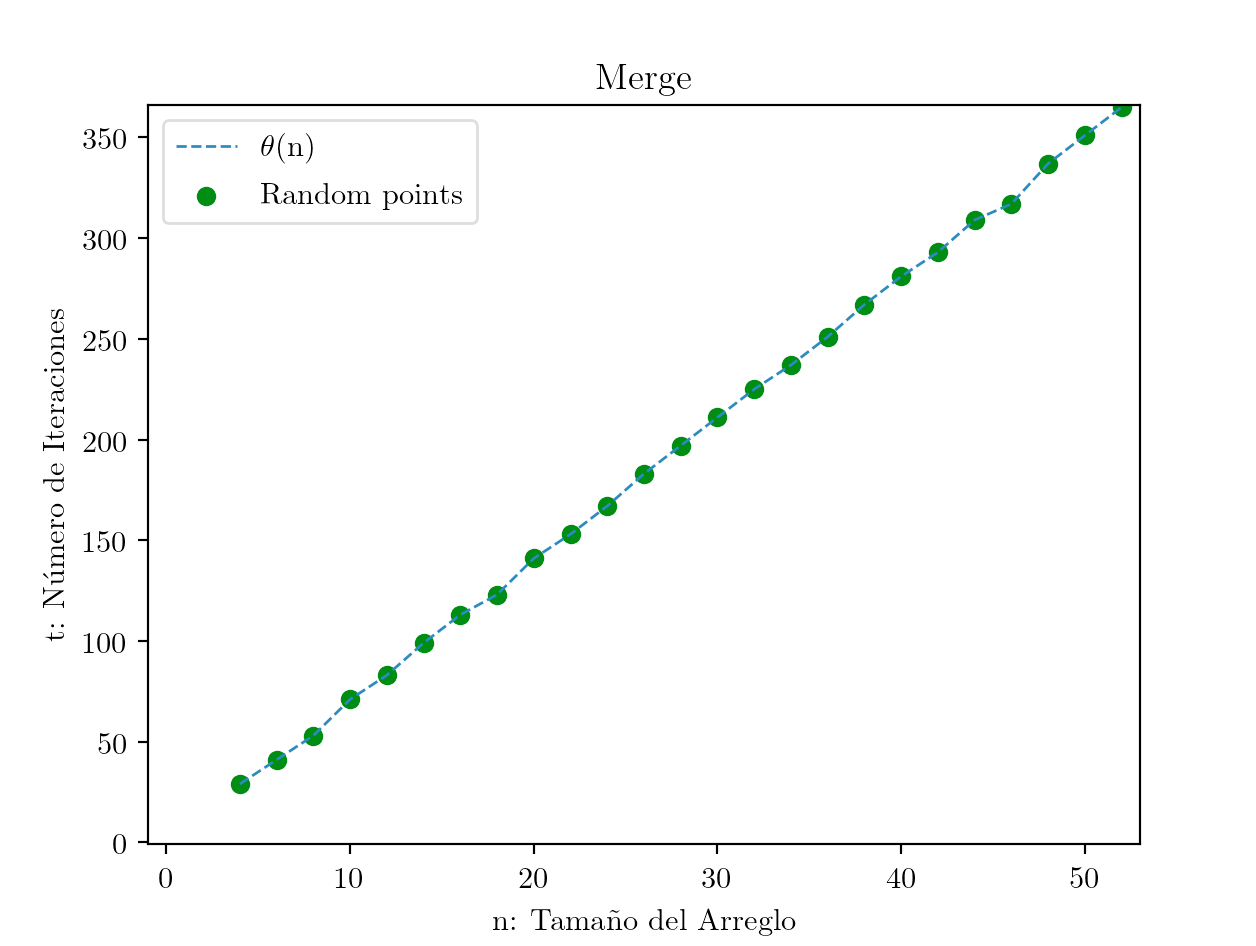
\includegraphics[height=0.5\textwidth]{Figure1}
  \caption{Comportamiento de Merge}
  \label{fig:ejemplo1}
\end{figure}

Sin embargo, se puede ver un comprotamiento inusual respecto a los whiles definidos dentro del else en la segunda mitad del algoritmo,
si lo analisamos detenidamente, la primera mitad del algoritmo($if$), puede recorrer $c = max\{i, j\} \mid I.length < i \lor D.length < j$,
como máximo, de tal manera que, al ingreso de la sentencia $else$ se recorre lo faltante respecto al tamaño del array $A$. Por lo tanto,
el recorrido en el $for$ hace un recorrido en con tamaño $r$, como máximo, independientemente de los whiles implementados. Por consiguiente,
graficando el número de iteracciones respecto al tamaño del array, se puede visualizar en la $(Figura$ $1)$, que se comporta como una recta.
Por lo tanto reafirmamos que el algoritmo de \textit{Merge} es lineal($T(n) \in O(n)$).


\subsection{\textbf{Soluci\'on al segundo problema}}

Para el desarrollo del algoritmo de \textit{Merge Sort}, es completamente necesario utilizar el algoritmo anterior \textit{Merge}, para que 
\textit{Merge Sort}, vaya dividiendo a la mitad, todos los elementos y \textit{Merge} los vaya ordenando, esto en términos sobre 
algoritmos, se dice que se aplica \textit{Divide y Vencerás}, donde la parte de Dividir la realiza el algoritmo de \textit{Merge Sort}, 
y el vencerás \textit{Merge}. Donde el algoritmo a proponer sería el \textbf{Algoritmo 2}.


\begin{algorithm}
  \caption{Merge Sort}
  \begin{algorithmic}[1]
  \Function{Merge Sort}{$A[0, ..., n-1], p, r$}
    \If{$p<r \land r \not = 0$} \Comment $O(1)$
      \State $q \gets \lfloor \frac{p + r}{2} \rfloor$ \Comment $O(1)$
      \State $Merge Sort(A,p,q)$ \Comment $T(\frac{n}{2})$
      \State $Merge Sort(A,q + 1,r)$ \Comment $T(\frac{n}{2})$
      \State $Merge(A,p,q,r)$ \Comment $O(n)$
    \EndIf
  \EndFunction
  \end{algorithmic}
\end{algorithm}

De acuerdo al análisis anterior del algoritmo de \textit{Merge} concluimos que tiene complejidad $O(n)$, entonces, para poder analizar 
el comportamiento del algoritmo de \textit{Merge Sort}, creamos su función de recurrencia.
\newpage
\begin{center}
  $T(n) =\left\{ \begin{array}{lcc}
      c_{1} &   si& n=1\\
  \\  2*T(\frac{n}{2}) + c_{2}*n &  si  & n>1 
  \end{array}
  \right.
  $
\end{center}

Debido a que no tenemos nocion acerca de $T(\frac{n}{2})$, optaremos por construir una nueva función de recurrencia a partir 
de la transformación $n = \log_{2} k \Rightarrow k = 2^n$. Entonces $T(n)$ en términos de $k$ sería:

\begin{center}
  $T(2^k) =\left\{ \begin{array}{lcc}
      c &   si& k=0\\
  \\  2*T(2^{k-1}) + c*2^k &  si  & k>0 
  \end{array}
  \right.
  $
\end{center}

Se tiene:\\

  $T(2^k)=2*T(2^{k-1}) + c*2^k$\\
  $T(2^k)=2*[2*T(2^{k-2}) + c*2^{k-1}] + c*2^k$\\
  $T(2^k)=2^2*T(2^{k-2}) + 2*c*2^k$\\
  $T(2^k)=2^2*[2*T(2^{k-3}) + c*2^{k-2}] + 2*c*2^k$\\
  $T(2^k)=2^3*T(2^{k-3}) + 3*c*2^k$\\
  $\vdots$\\
  $T(2^k)=2^i*T(2^{k-i}) + i*c*2^k$\\ 
  \centerline{}
  Si $k = i$, entonces:\\
  $T(2^k)=2^k*T(1) + k*c*2^k$\\ 
  \centerline{}
  Regresando a $n$:\\
  $T(n)=n*T(1) + \log_{2}(n)*c*n$\\
  $\therefore T(n) \in O(n \log(n))$\\ \\

\begin{figure}
  \centering
    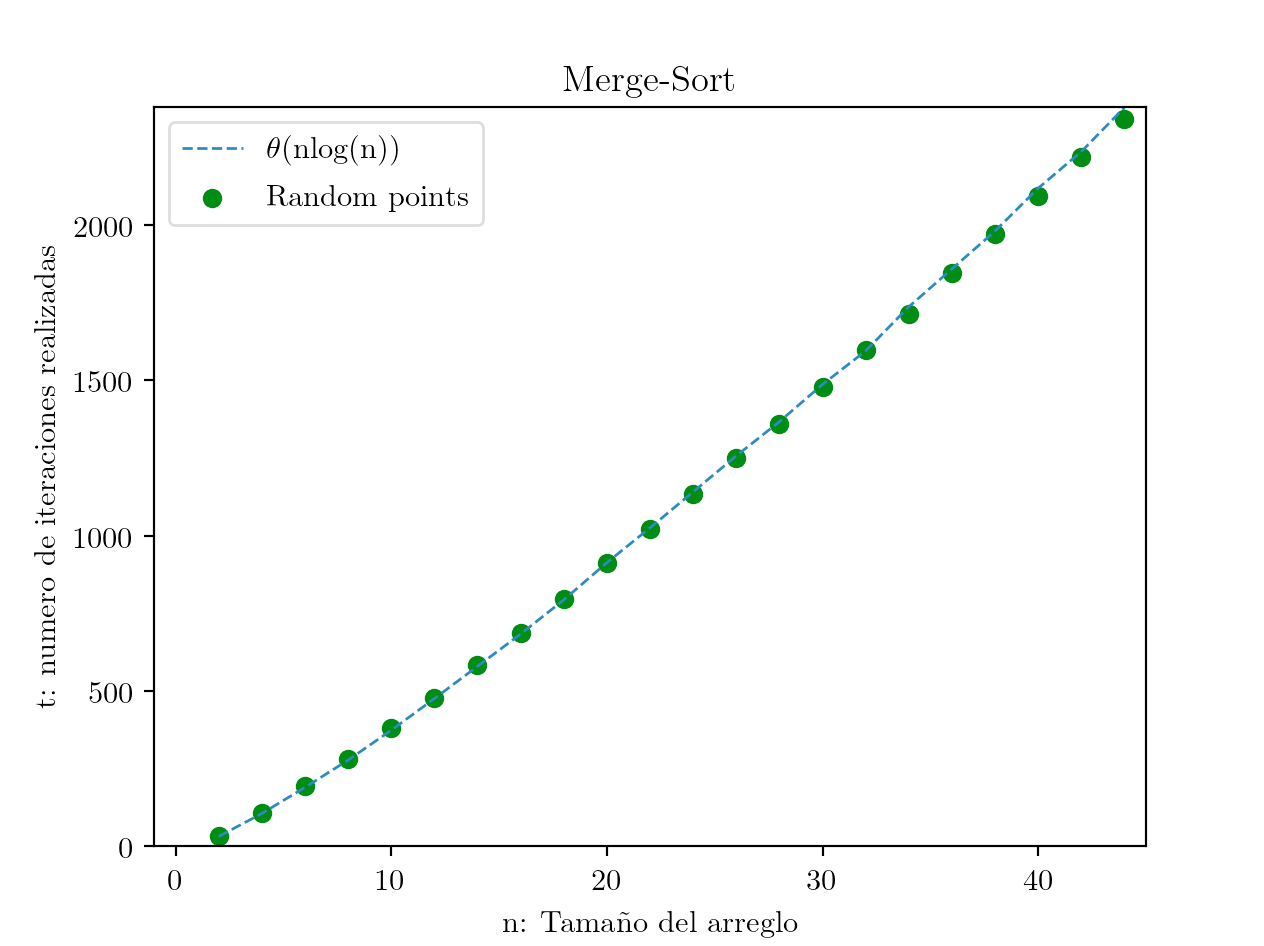
\includegraphics[height=0.5\textwidth]{Figure2}
  \caption{Comportamiento de Merge Sort}
  \label{fig:ejemplo3}
\end{figure}

Podemos decir que la función \textit{Merge Sort}, tiene una complegitada $n \log(n)$ la cual podemos reforzar aún más mediante el 
método grafico entre las iteraciones realizadas respecto del tamaño del array $(Figura$ $2)$. Aunque en la gráfica parezca que 
el algoritmo sea lineal, realmente no, al acercase puede verse una pequeña curva, incluso si pretendemos determinar la pendiente,
si fuese una recta, con cada par de puntos nos darían resultados diferentes. En tanto, concluímos que \textit{Merge Sort} $\in O(n \log(n))$

\newpage

\section{Anexo} 
\text{}\\ 
\textbf{Cálculo del orden de complejidad de dos funciones, de las cuales se debe verificar cuales son el peor y el mejor de los casos}\\ \begin{algorithm}

\caption{Funcion 1}\label{euclid}
\begin{algorithmic}[1]
  \Function{Funcion 1}{$n$ par} 
    \While{$i<n$} \Comment O(n)
      \For{$j=0$ \textbf{to} $j=10$} \Comment O(n)
          \State $Accion(i)$  \Comment O(1)
          \State \textbf{$j++$} \Comment O(1)   
      \EndFor
      \State \textit{$i += 2$}  \Comment O(1)    
    \EndWhile
  \EndFunction
\end{algorithmic}
\end{algorithm}

Este algoritmo tiene complejidad en el peor de los casos de $O(n)$ y en el mejo de los casos es cuando n no es par y no entra en el algoritmo por lo tanto es $\Omega (1)$
\newpage
\begin{algorithm}
\caption{Funcion 2}\label{euclid}
  \begin{algorithmic}[2]
  \Function{Funcion2}{$A[0,...,n-1],x$ entero} 
    \For{$i=0$ \textbf{to} $i<n$} \Comment O(n)
      \If{$A[i]<x$}\Comment O(1) 
        \State $A[i]=min(A[0,...,n-1])$ \Comment O(n) 
      \ElsIf{$A[i]>x$} \Comment O(1) 
        \State$A[i]=max(A[0,...,n-1])$ \Comment O(n) 
      \Else
        \State \textbf{$exit$} \Comment O(1) 
      \EndIf
    \EndFor
  \EndFunction
  \end{algorithmic}
\end{algorithm}

Este algoritmo tiene la misma complejidad en el peor y en el mejor de lo casos por lo tanto esu complejidad es $\Theta (n^2)$



\newpage
\section{Conclusiones}
\textbf{Conclusion Alejandro Contreras Paredes}\\
En esta practica se encontro que los algoritmos empleadso para la codificaci\'on de los mismos no estaba completo, el cual represento un problema
que conllevo a un retraso significativo de las demas partes que la componian, pero con esfuerzo se pudo resolver y continuar.
Resulta curioso como 2 algoritmos se pueden relacionar entre s\'i y formar algo que es de mayor utilidad pero tambien hay que tomar en cuenta 
que esta relaci\'on puede significar un aumento en el costo computacional. Finalmente, con los conocimientos obtenidos se pudo realizar la practica en tiempo.
\\\\
\textbf{Conclusion Fernando Daniel Rivera Paredes}\\

En el desarrollo de la práctica, tuvimos un primer percance respecto al algoritmo de Merge, debido a que esta incompleto, y faltaba un manejo
correcto de los indices al desbordamiento de los índices, estuvo muy bien el manejo ante esa "trampa`` en el código, para que uno como alumno
autodidacta pretenda realizar una solución sin afectar la complejidad del algoritmo. Finalmente, la parte gráfica solía ser muy confusa al inicio
dado que no se podía visualizar correctamente las curvas que mostraban. 
\begin{figure}[!h]
	\centering
	\begin{minipage}[t]{10cm}
		\centering
		
\includegraphics[scale=0.2]{Foto1}
		\caption{Alejandro Contreras Paredes}
	\end{minipage}
	\hspace{18cm}
	\begin{minipage}[t]{10cm}
		\centering
		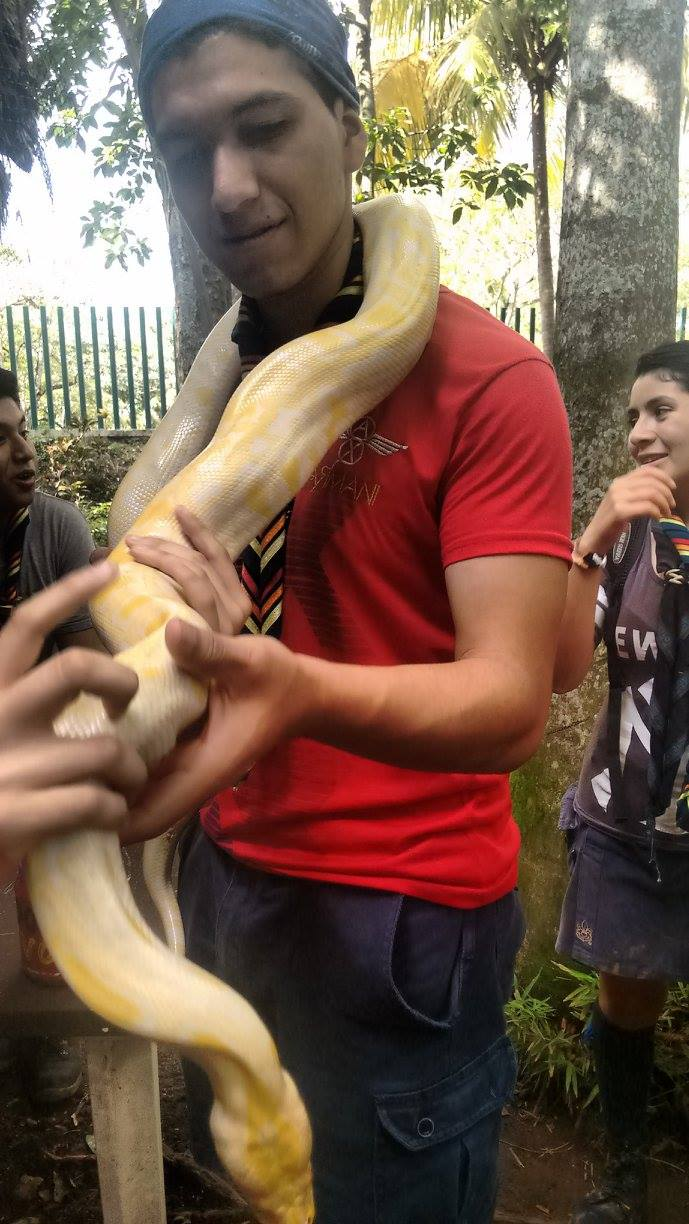
\includegraphics[scale=0.2]{Foto2}
		\caption{Rivera Paredes Fernando Daniel}
	\end{minipage}
\end{figure}

\section{Bibliograf\'ia}

\begin{thebibliography}{9}
  \bibitem{book} 
  Cormen, T. and Leiserson, C.
  \textit{Introduction to algorithms.} 
  3rd edition.Cambridge, Massachusetts: Massachusetts Institute of Technology, 2009.

  \bibitem{ie} 
  Moyano, N.
  \textit{Análisis de algoritmos}.
  Medium. Available at: $www.lcc.uma.es/~av/Libro/CAP3.pdf$'[Accessed 03 Sep. 2019].
\end{thebibliography}
\end{document}
